\documentclass[tikz,dvipsnames]{standalone}
\usetikzlibrary{calc,quotes}
\usetikzlibrary{backgrounds, shapes,automata,patterns}

\boldmath
\normalsize

\newcommand{\blank}{\sqcup}

\tikzset{
  bg/.style = {fill=white,line width=1, draw=black},
  state/.style = {circle,draw=black,fill=white,line width=1.5,inner sep=0pt,minimum size=25pt},
  every initial by arrow/.style={draw=none},
  initial distance=-0.09cm,
  initial text = {\Huge\color{black} $>$},
   current/.style ={circle,draw=black,fill=white,line width=1.5,inner sep=0pt,minimum size=25pt,pattern=north east lines},
   %
   edge/.style = {->,>=stealth,line width=2,>=latex,black,text=black},
   active/.style = {circle,draw=black,fill=white,line width=3,inner sep=0pt,minimum size=25pt,pattern=north west lines},
   rejecting/.style = {accepting},
  last edge/.style = {->,>=stealth,line width=4,>=latex,draw=black},
}


\begin{document}
  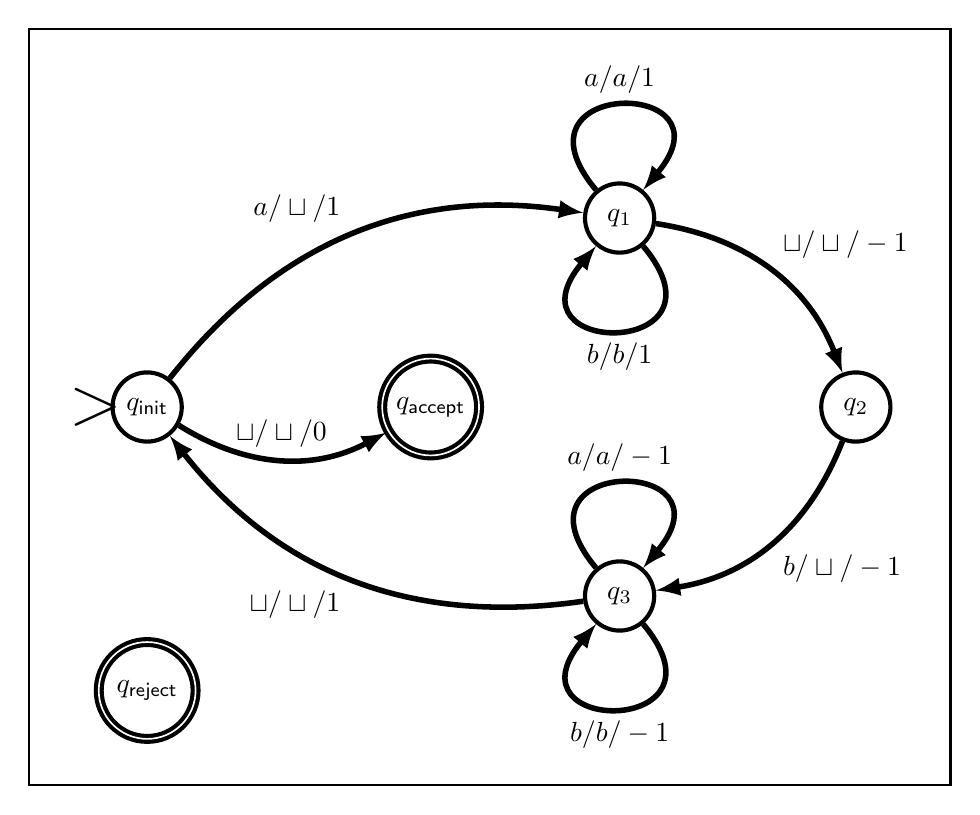
\begin{tikzpicture}[yscale=3,xscale=3]
    \draw[bg] (-0.5,-1.6) rectangle (3.4,1.6) ;

    \node[state,initial] at (0,0) (init) {$q_{\mathsf{init}}$};
    \node[state] at (2,0.8) (q1) {$q_1$};
    \node[state,accepting,minimum size=35pt] at (1.2,0) (accept) {$q_{\mathsf{accept}}$};
    \node[state] at (3,0) (q2) {$q_2$};
    \node[state] at (2,-0.8) (q3) {$q_3$};
    \node[state,rejecting,minimum size=35pt] at (0,-1.2) (reject) {$q_{\mathsf{reject}}$};


    \draw[edge, bend left] (init) to node[above left] {$a/\blank/1$} (q1);

    \draw[edge, bend right] (init) to node[above] {$\blank/\blank/0$} (accept);

    \draw[edge, bend left] (q1) to node[above right,text=black] {$\blank/\blank/-1$} (q2);

    \draw[edge, bend left] (q2) to node[below right,text=black] {$b/\blank/-1$} (q3);
    \draw[edge, bend left] (q3) to node[below left,text=black] {$\blank/\blank/1$} (init);

    \draw[edge,looseness=8, in=50, out=130] (q1) to node[above,text=black] {$a/a/1$} (q1);
    \draw[edge,looseness=8, in=-130, out=-50] (q1) to node[below,text=black] {$b/b/1$} (q1);

    \draw[edge,looseness=8, in=50, out=130] (q3) to node[above,text=black] {$a/a/-1$} (q3);
    \draw[edge,looseness=8, in=-130, out=-50] (q3) to node[below,text=black] {$b/b/-1$} (q3);


\end{tikzpicture}
\end{document}
